\subsection{Implementation Plan}

The implementation plan defines the sequential steps for developing the system's components, ensuring that each feature and module is designed, developed, and tested effectively. The Bottom-Up methodology will be used to break down the entire system into simplest possible subsystems that recursively build up to the required solution. Each component will follow the Single Responsibility Principle (SRP) and will be implemented using Test-Driven Development (TDD).

\subsubsection{Development of Core Components}

\paragraph{User Authentication and Profile Management:}
The objective is to implement secure registration and login functionalities for students, companies, and universities, with each user type having their own profile and corresponding data. To achieve this, we will develop the user registration functionality, allowing for input of name, email, password, and role selection. We will also implement login and session management to ensure secure access. Each user type will be able to create and edit their profile, with students entering their academic and experience details, while companies provide internship descriptions. For this, we will use OAuth 2.0 for secure authentication and PostgreSQL/MySQL for storing user data.

\begin{figure}[H]
\centering
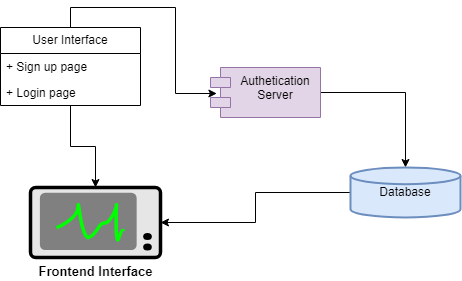
\includegraphics[width=0.8\textwidth]{Images/core1.png}
\caption{User Authentication and Profile Management.}
\end{figure}

\paragraph{Internship Search and Application System:}
The objective of this component is to provide students with a way to search for, view, and apply for internships. This will involve developing a search functionality that uses filters like location, skills, and internship type. The system will display relevant internship details such as job descriptions, company names, and locations. Students will also have the option to apply directly to internships by clicking the "Apply" button. Elasticsearch will be used to index and search internship listings, and we will integrate this functionality with the backend API to display search results in real-time.

\begin{figure}[H]
\centering
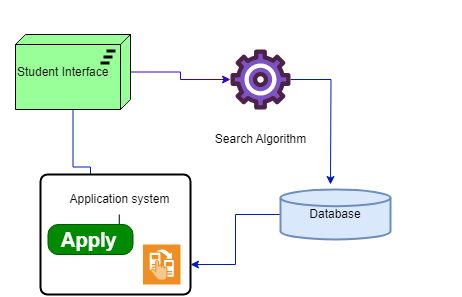
\includegraphics[width=0.8\textwidth]{Images/core2.png}
\caption{Internship Search and Application System.}
\end{figure}

\paragraph{Internship Posting:}
Companies will be able to post internships, and the system will automatically match students with relevant positions based on their profiles. To implement this, we will create the "Post Internship" functionality, which will allow companies to add internship roles. The frontend for posting the internship details will show writing improvement suggestions to the author to increase the likelihood of finding suitable matches with Student profiles. The backend service will be developed using Node.js.
The system will use the Recommendation Engine described below to recommend internships to students, based on their profile data, such as skills, experience, and location preferences.

\paragraph{Recommendation/Matching Engine:}
 The Recommendation/Matching Engine will run as a Cron Job at regular intervals of 24 hours for each Student to identify Internships relevant to their skills and background. In order to achieve performance optimization, an Embedding will be calculated ahead-of-time for each Student profile using a Neural Network trained on anonymized data of past Student profile and Internship matches. The Neural Network will use Matrix Factorization to learn the representation of Latent Factors from the available profile and internship attributes and create the Embedding. This Embedding will be re-calculated whenever a Student updates any attributes of their profile. The Recommendation/Matching Engine will use a Model-Based Collaborative Filtering (MCBF) to match new Student profiles to Internships based on the pre-calculated Embeddings to optimize compute resource utilization. The system will use the Notification Manager to alert both students and companies about new matches. The backend logic will be developed using Python, and machine learning algorithms will be applied for the matching process.

\begin{figure}[H]
\centering
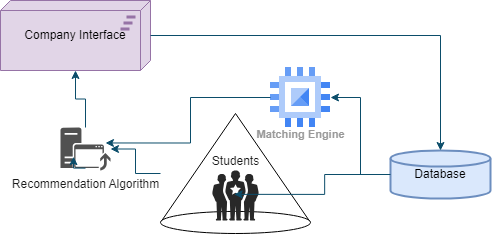
\includegraphics[width=0.8\textwidth]{Images/core3.png}
\caption{Internship Posting and Matching Engine.}
\end{figure}

\paragraph{Interview Scheduling and Feedback Collection:}
The system will support companies in scheduling interviews with selected candidates and collecting feedback after the interview. The interview scheduling tool will allow students and companies to select available time slots. Integration with a video conferencing system like Zoom will allow for virtual interviews, and the system will also collect feedback after each interview. For scheduling, we will use the Google Calendar API, and Zoom will be integrated for video calls. The feedback system will be custom-built to collect and store feedback from both students and companies.

\begin{figure}[H]
\centering
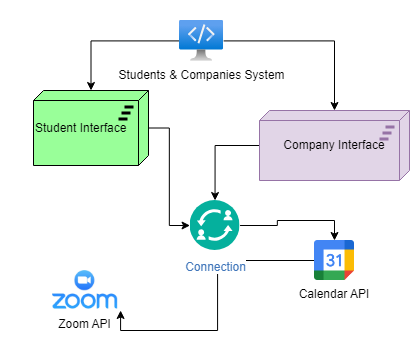
\includegraphics[width=0.8\textwidth]{Images/core42.png}
\caption{Interview Scheduling.}
\end{figure}
\begin{figure}[H]
\centering
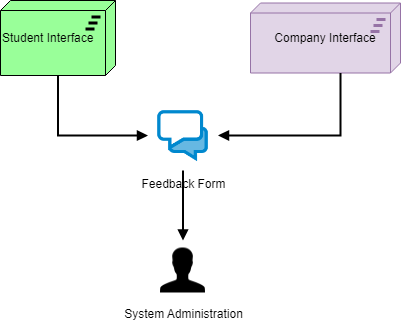
\includegraphics[width=0.8\textwidth]{Images/core41.png}
\caption{Feedback Collection.}
\end{figure}

\paragraph{Complaint Handling and University Monitoring System:}
This component will enable universities to monitor student internship progress and handle complaints from both students and companies. Universities will be able to track the status of all students' internship applications using a dedicated dashboard. A complaint reporting and resolution workflow will be developed to allow students and companies to raise and resolve issues. Notifications will be sent to the involved parties (students, companies, universities), and the university will oversee the resolution process. The notification system will be built using email or push notifications, and the interface for universities will be user-friendly and easily accessible.

\begin{figure}[H]
\centering
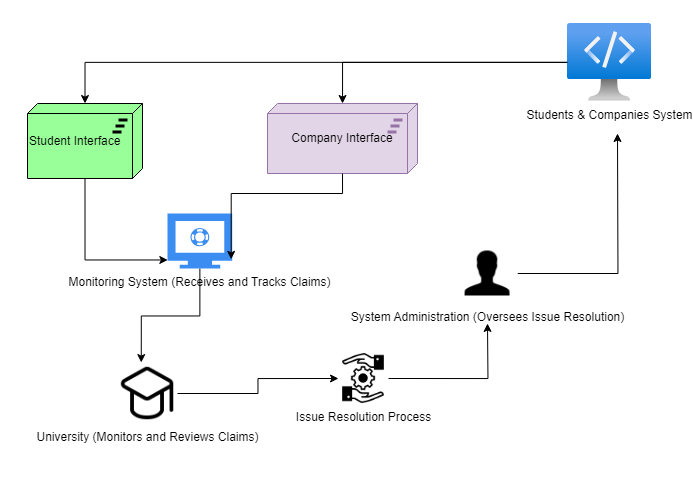
\includegraphics[width=0.8\textwidth]{Images/core5.png}
\caption{Complaint Handling and University Monitoring System.}
\end{figure}

\subsubsection{Technology Stack}

\begin{itemize}
    \item \textbf{Frontend:} ReactJS or Angular will be used to build responsive and interactive user interfaces.
    \item \textbf{Backend:} Node.js with Express.js or Django will handle business logic and REST API services.
    \item \textbf{Database:} PostgreSQL or MySQL will store structured data such as user profiles, internship listings, and applications.
    \item \textbf{Search Engine:} Elasticsearch will be used for indexing and filtering internship listings efficiently.
    \item \textbf{Recommendation System:} Python or JavaScript-based machine learning models will be used for matching students with internships.
    \item \textbf{Video Conferencing:} Zoom API will be integrated for virtual interviews.
    \item \textbf{Notification System:} Email services like NodeMailer or SendGrid will be used for sending user notifications.
\end{itemize}

\subsection{Integration Plan}

Once the core components are developed, we will proceed with the integration phase. This phase involves combining the various subsystems, ensuring smooth data flow, and confirming that all functionalities work together.

\subsubsection{Integration of User Authentication and Profile Management}
The user authentication system will be integrated with the frontend, allowing users to sign up, log in, and access their profile pages. Role-based views (Student, Company, University) will be displayed based on the user’s role.

\subsubsection{Integration of Internship Search and Application System}
The search functionality will be connected to the backend to fetch real-time data, and the "Apply" functionality will be integrated to submit student applications to companies.

\subsubsection{Integration of Internship Posting and Matching Engine}
Companies will be able to post internships, and the system will match these postings with student profiles. The matching engine will use the student’s profile data to recommend internships, and notifications will inform both students and companies about new matches.

\subsubsection{Integration of Interview Scheduling and Feedback Collection}
The interview scheduling feature will be integrated, allowing both students and companies to select available time slots. Zoom integration will ensure video meetings, and feedback will be collected and stored after interviews.

\subsubsection{Integration of Complaint Handling and University Monitoring}
Universities will be able to monitor the internship status of students and resolve complaints through the system. The complaint submission and resolution process will be integrated, and notifications will inform all relevant parties.

\subsubsection{End-to-End Testing}
We will ensure that data flows seamlessly between the frontend, backend, and database. Additionally, we will test for any UI/UX issues and resolve any discrepancies. Unit tests for individual components and integration tests for interactions between modules will be conducted.

\subsection{Testing Plan}

Testing will be done iteratively during development, followed by extensive system testing to ensure robustness and correctness.

\subsubsection{Unit Testing}
The goal is to verify that individual components, such as user authentication, profile creation, internship search, matching algorithm, and interview scheduling, work correctly.

\subsubsection{Integration Testing}
We will verify that the components work together seamlessly. For example, we will check if user registration leads to successful login and profile creation, if students can apply for internships, and if the matching system works as intended.

\subsubsection{Functional Testing}
This type of testing will ensure that the system meets all functional requirements. Students should be able to search for internships, companies should be able to post internships, and universities should be able to monitor student progress and handle complaints.

\subsubsection{Performance Testing}
We will conduct load testing to simulate multiple users accessing the system simultaneously. We will also test the system’s response time and performance under peak usage conditions.

\subsubsection{Security Testing}
The security of the platform will be tested to ensure that user credentials are encrypted, and the system is protected against common security threats such as SQL injection and XSS attacks.

\subsubsection{Technology Stack}

\begin{itemize}
    \item \textbf{Testing Tools:} Jest or Mocha for unit testing the individual components of the system.
    \item \textbf{Integration Testing Tools:} Postman or Supertest for testing REST API integrations between frontend and backend.
    \item \textbf{Performance Testing:} Apache JMeter or LoadRunner for conducting load and performance tests.
    \item \textbf{Security Testing:} OWASP ZAP or Burp Suite for vulnerability scanning and security testing.
\end{itemize}

\subsubsection{User Acceptance Testing (UAT)}
Actual users (students, companies, universities) will test the system to ensure it meets their needs. Feedback will be collected, and any necessary adjustments will be made before deployment.
